\documentclass{article}

\usepackage[utf8]{inputenc}
\usepackage{hyperref}
\usepackage{amsmath}
\usepackage{amssymb}
\usepackage{amsthm}
\usepackage{isabelle}
\usepackage{isabellesym}
\usepackage{algpseudocode}
\usepackage{tikz}
\usepackage{stmaryrd}
\usepackage{ifthen}

\newcommand{\iassert}[1]{\mathtt{Assert}(#1)}
\newcommand{\icheck}{\mathtt{Check}()}
\newcommand{\icheckpoint}{\mathtt{Checkpoint}()}
\newcommand{\ibacktrack}[1]{\mathtt{Backtrack}(#1)}
%\newcommand{\csat}{\mathtt{Satisfiable}}
\newcommand{\cunsat}{\texttt{Unsatisfiable}}
\newcommand{\cone}{\mathrm{cone}}
\newcommand{\hull}{\mathrm{hull}}
\newcommand{\ints}{\mathbb{Z}}
\newcommand{\ifff}{if and only if}

% Source: https://isabelle.in.tum.de/community/Generate_TeX_Snippets
\newcommand{\DefineSnippet}[2]{%
  \expandafter\newcommand\csname snippet--#1\endcsname{%
    \begin{quote}
    \begin{isabelle}
    #2
    \end{isabelle}
    \end{quote}}}
\newcommand{\Snippet}[1]{%
  \ifcsname snippet--#1\endcsname{\csname snippet--#1\endcsname}%
  \else+++++++ERROR: Snippet ``#1 not defined+++++++ \fi}

\DefineSnippet{cantor}{
\isacommand{lemma}\isamarkupfalse%
\ {\isachardoublequoteopen}{\isasymnot}\ surj\ {\isacharparenleft}f\ {\isacharcolon}{\isacharcolon}\ {\isacharprime}a\ {\isasymRightarrow}\ {\isacharprime}a\ set{\isacharparenright}{\isachardoublequoteclose}\isanewline
%
\isadelimproof
%
\endisadelimproof
%
\isatagproof
\isacommand{proof}\isamarkupfalse%
\isanewline
\ \ \isacommand{assume}\isamarkupfalse%
\ {\isachardoublequoteopen}surj\ f{\isachardoublequoteclose}\isanewline
\ \ \isacommand{hence}\isamarkupfalse%
\ {\isachardoublequoteopen}{\isasymexists}\ a{\isachardot}\ {\isacharbraceleft}x{\isachardot}\ x\ {\isasymnotin}\ f\ x{\isacharbraceright}\ {\isacharequal}\ f\ a{\isachardoublequoteclose}\ \isacommand{by}\isamarkupfalse%
\ blast\isanewline
\ \ \isacommand{thus}\isamarkupfalse%
\ False\ \isacommand{by}\isamarkupfalse%
\ auto\isanewline
\isacommand{qed}\isamarkupfalse%
%
\endisatagproof
{\isafoldproof}%
%
\isadelimproof
%
\endisadelimproof
%
}%EndSnippet

\DefineSnippet{nonneg-lincomb}{
\isacommand{definition}\isamarkupfalse%
\ {\isachardoublequoteopen}nonneg{\isacharunderscore}lincomb\ c\ Vs\ b\ {\isacharequal}\isanewline
\ \ {\isacharparenleft}lincomb\ c\ Vs\ {\isacharequal}\ b\ {\isasymand}\ c\ {\isacharbackquote}\ Vs\ {\isasymsubseteq}\ {\isacharbraceleft}x{\isachardot}\ x\ {\isasymge}\ {\isadigit{0}}{\isacharbraceright}{\isacharparenright}{\isachardoublequoteclose}%
}%EndSnippet
\DefineSnippet{nonneg-lincomb-list}{
\isacommand{definition}\isamarkupfalse%
\ {\isachardoublequoteopen}nonneg{\isacharunderscore}lincomb{\isacharunderscore}list\ c\ Vs\ b\ {\isacharequal}\isanewline
\ \ {\isacharparenleft}lincomb{\isacharunderscore}list\ c\ Vs\ {\isacharequal}\ b\ {\isasymand}\ {\isacharparenleft}{\isasymforall}\ i\ {\isacharless}\ length\ Vs{\isachardot}\ c\ i\ {\isasymge}\ {\isadigit{0}}{\isacharparenright}{\isacharparenright}{\isachardoublequoteclose}%
}%EndSnippet
\DefineSnippet{finite-cone}{
\isacommand{definition}\isamarkupfalse%
\ finite{\isacharunderscore}cone\ {\isacharcolon}{\isacharcolon}\ {\isachardoublequoteopen}{\isacharprime}a\ vec\ set\ {\isasymRightarrow}\ {\isacharprime}a\ vec\ set{\isachardoublequoteclose}\ \isakeyword{where}\isanewline
\ \ {\isachardoublequoteopen}finite{\isacharunderscore}cone\ Vs\ {\isacharequal}\ {\isacharparenleft}{\isacharbraceleft}\ b{\isachardot}\ {\isasymexists}\ c{\isachardot}\ nonneg{\isacharunderscore}lincomb\ c\ {\isacharparenleft}if\ finite\ Vs\ then\ Vs\ else\ {\isacharbraceleft}{\isacharbraceright}{\isacharparenright}\ b{\isacharbraceright}{\isacharparenright}{\isachardoublequoteclose}%
}%EndSnippet
\DefineSnippet{cone}{
\isacommand{definition}\isamarkupfalse%
\ cone\ {\isacharcolon}{\isacharcolon}\ {\isachardoublequoteopen}{\isacharprime}a\ vec\ set\ {\isasymRightarrow}\ {\isacharprime}a\ vec\ set{\isachardoublequoteclose}\ \isakeyword{where}\isanewline
\ \ {\isachardoublequoteopen}cone\ Vs\ {\isacharequal}\ {\isacharparenleft}{\isacharbraceleft}\ x{\isachardot}\ {\isasymexists}\ Ws{\isachardot}\ finite\ Ws\ {\isasymand}\ Ws\ {\isasymsubseteq}\ Vs\ {\isasymand}\ x\ {\isasymin}\ finite{\isacharunderscore}cone\ Ws{\isacharbraceright}{\isacharparenright}{\isachardoublequoteclose}%
}%EndSnippet
\DefineSnippet{cone-list}{
\isacommand{definition}\isamarkupfalse%
\ cone{\isacharunderscore}list\ {\isacharcolon}{\isacharcolon}\ {\isachardoublequoteopen}{\isacharprime}a\ vec\ list\ {\isasymRightarrow}\ {\isacharprime}a\ vec\ set{\isachardoublequoteclose}\ \isakeyword{where}\isanewline
\ \ {\isachardoublequoteopen}cone{\isacharunderscore}list\ Vs\ {\isacharequal}\ {\isacharbraceleft}b{\isachardot}\ {\isasymexists}c{\isachardot}\ nonneg{\isacharunderscore}lincomb{\isacharunderscore}list\ c\ Vs\ b{\isacharbraceright}{\isachardoublequoteclose}%
}%EndSnippet
\DefineSnippet{finite-cone-iff-cone-list}{
\isacommand{lemma}\isamarkupfalse%
\ finite{\isacharunderscore}cone{\isacharunderscore}iff{\isacharunderscore}cone{\isacharunderscore}list{\isacharcolon}\ \isakeyword{assumes}\ Vs{\isacharcolon}\ {\isachardoublequoteopen}Vs\ {\isasymsubseteq}\ carrier{\isacharunderscore}vec\ n{\isachardoublequoteclose}\isanewline
\ \ \isakeyword{and}\ id{\isacharcolon}\ {\isachardoublequoteopen}Vs\ {\isacharequal}\ set\ Vsl{\isachardoublequoteclose}\isanewline
\isakeyword{shows}\ {\isachardoublequoteopen}finite{\isacharunderscore}cone\ Vs\ {\isacharequal}\ cone{\isacharunderscore}list\ Vsl{\isachardoublequoteclose}%
}%EndSnippet
\DefineSnippet{convex-lincomb}{
\isacommand{definition}\isamarkupfalse%
\ {\isachardoublequoteopen}convex{\isacharunderscore}lincomb\ c\ Vs\ b\ {\isacharequal}\isanewline
\ \ {\isacharparenleft}nonneg{\isacharunderscore}lincomb\ c\ Vs\ b\ {\isasymand}\ sum\ c\ Vs\ {\isacharequal}\ {\isadigit{1}}{\isacharparenright}{\isachardoublequoteclose}%
}%EndSnippet
\DefineSnippet{convex-lincomb-list}{
\isacommand{definition}\isamarkupfalse%
\ {\isachardoublequoteopen}convex{\isacharunderscore}lincomb{\isacharunderscore}list\ c\ Vs\ b\ {\isacharequal}\isanewline
\ \ {\isacharparenleft}nonneg{\isacharunderscore}lincomb{\isacharunderscore}list\ c\ Vs\ b\ {\isasymand}\ sum\ c\ {\isacharbraceleft}{\isadigit{0}}{\isachardot}{\isachardot}{\isacharless}length\ Vs{\isacharbraceright}\ {\isacharequal}\ {\isadigit{1}}{\isacharparenright}{\isachardoublequoteclose}%
}%EndSnippet
\DefineSnippet{convex-hull}{
\isacommand{definition}\isamarkupfalse%
\ {\isachardoublequoteopen}convex{\isacharunderscore}hull\ Vs\ {\isacharequal}\isanewline
\ \ {\isacharbraceleft}x{\isachardot}\ {\isasymexists}\ Ws\ c{\isachardot}\ finite\ Ws\ {\isasymand}\ Ws\ {\isasymsubseteq}\ Vs\ {\isasymand}\ convex{\isacharunderscore}lincomb\ c\ Ws\ x{\isacharbraceright}{\isachardoublequoteclose}%
}%EndSnippet
\DefineSnippet{convex-hull-list}{
\isacommand{definition}\isamarkupfalse%
\ {\isachardoublequoteopen}convex{\isacharunderscore}hull{\isacharunderscore}list\ Vs\ {\isacharequal}\isanewline
\ \ {\isacharbraceleft}x{\isachardot}\ {\isasymexists}\ c{\isachardot}\ convex{\isacharunderscore}lincomb{\isacharunderscore}list\ c\ Vs\ x{\isacharbraceright}{\isachardoublequoteclose}%
}%EndSnippet
\DefineSnippet{convex-hull-equivalence}{
\isacommand{lemma}\isamarkupfalse%
\ finite{\isacharunderscore}convex{\isacharunderscore}hull{\isacharunderscore}iff{\isacharunderscore}convex{\isacharunderscore}hull{\isacharunderscore}list{\isacharcolon}\isanewline
\ \ \isakeyword{assumes}\ Vs{\isacharcolon}\ {\isachardoublequoteopen}Vs\ {\isasymsubseteq}\ carrier{\isacharunderscore}vec\ n{\isachardoublequoteclose}\isanewline
\ \ \isakeyword{and}\ id{\isacharprime}{\isacharcolon}\ {\isachardoublequoteopen}Vs\ {\isacharequal}\ set\ Vsl{\isacharprime}{\isachardoublequoteclose}\isanewline
\isakeyword{shows}\ {\isachardoublequoteopen}convex{\isacharunderscore}hull\ Vs\ {\isacharequal}\ convex{\isacharunderscore}hull{\isacharunderscore}list\ Vsl{\isacharprime}{\isachardoublequoteclose}%
}%EndSnippet
\DefineSnippet{farkas-minkowsky-1}{
\isacommand{lemma}\isamarkupfalse%
\ farkas{\isacharunderscore}minkowsky{\isacharunderscore}weyl{\isacharunderscore}theorem{\isacharunderscore}{\isadigit{1}}{\isacharcolon}\isanewline
\ \ \isakeyword{assumes}\ X{\isacharcolon}\ {\isachardoublequoteopen}X\ {\isasymsubseteq}\ carrier{\isacharunderscore}vec\ n{\isachardoublequoteclose}\isanewline
\ \ \ \ \isakeyword{and}\ finX{\isacharcolon}\ {\isachardoublequoteopen}finite\ X{\isachardoublequoteclose}\isanewline
\ \ \isakeyword{shows}\ {\isachardoublequoteopen}{\isasymexists}\ nr\ A{\isachardot}\ A\ {\isasymin}\ carrier{\isacharunderscore}mat\ nr\ n\ {\isasymand}\ cone\ X\ {\isacharequal}\ polyhedral{\isacharunderscore}cone\ A\ {\isasymand}\isanewline
\ \ \ \ {\isacharparenleft}X\ {\isasymsubseteq}\ {\isasymint}\isactrlsub v\ {\isasyminter}\ Bounded{\isacharunderscore}vec\ Bnd\ {\isasymlongrightarrow}\ A\ {\isasymin}\ {\isasymint}\isactrlsub m\ {\isasyminter}\ Bounded{\isacharunderscore}mat\ {\isacharparenleft}det{\isacharunderscore}bound\ {\isacharparenleft}n{\isacharminus}{\isadigit{1}}{\isacharparenright}\ {\isacharparenleft}max\ {\isadigit{1}}\ Bnd{\isacharparenright}{\isacharparenright}{\isacharparenright}{\isachardoublequoteclose}%
}%EndSnippet
\DefineSnippet{farkas-minkowsky-2}{
\isacommand{lemma}\isamarkupfalse%
\ farkas{\isacharunderscore}minkowsky{\isacharunderscore}weyl{\isacharunderscore}theorem{\isacharunderscore}{\isadigit{2}}{\isacharcolon}\isanewline
\ \ \isakeyword{assumes}\ A{\isacharcolon}\ {\isachardoublequoteopen}A\ {\isasymin}\ carrier{\isacharunderscore}mat\ nr\ n{\isachardoublequoteclose}\isanewline
\ \ \isakeyword{shows}\ {\isachardoublequoteopen}{\isasymexists}\ X{\isachardot}\ X\ {\isasymsubseteq}\ carrier{\isacharunderscore}vec\ n\ {\isasymand}\ finite\ X\isanewline
\ \ \ \ \ \ \ \ \ \ \ \ {\isasymand}\ polyhedral{\isacharunderscore}cone\ A\ {\isacharequal}\ cone\ X\isanewline
\ \ {\isasymand}\ {\isacharparenleft}A\ {\isasymin}\ {\isasymint}\isactrlsub m\ {\isasyminter}\ Bounded{\isacharunderscore}mat\ Bnd\ {\isasymlongrightarrow}\isanewline
\ \ \ \ \ X\ {\isasymsubseteq}\ {\isasymint}\isactrlsub v\ {\isasyminter}\ Bounded{\isacharunderscore}vec\ {\isacharparenleft}det{\isacharunderscore}bound\ {\isacharparenleft}n{\isacharminus}{\isadigit{1}}{\isacharparenright}\ {\isacharparenleft}max\ {\isadigit{1}}\ Bnd{\isacharparenright}{\isacharparenright}{\isacharparenright}{\isachardoublequoteclose}%
}%EndSnippet
\DefineSnippet{farkas-minkowsky}{
\isacommand{lemma}\isamarkupfalse%
\ farkas{\isacharunderscore}minkowsky{\isacharunderscore}weyl{\isacharunderscore}theorem{\isacharcolon}\isanewline
\ \ {\isachardoublequoteopen}{\isacharparenleft}{\isasymexists}\ X{\isachardot}\ X\ {\isasymsubseteq}\ carrier{\isacharunderscore}vec\ n\ {\isasymand}\ finite\ X\ {\isasymand}\ P\ {\isacharequal}\ cone\ X{\isacharparenright}\isanewline
\ \ {\isasymlongleftrightarrow}\ {\isacharparenleft}{\isasymexists}\ A\ nr{\isachardot}\ A\ {\isasymin}\ carrier{\isacharunderscore}mat\ nr\ n\ {\isasymand}\ P\ {\isacharequal}\ polyhedral{\isacharunderscore}cone\ A{\isacharparenright}{\isachardoublequoteclose}%
}%EndSnippet

\DefineSnippet{satisfies-mixed}{
\isacommand{fun}\isamarkupfalse%
\ satisfies{\isacharunderscore}mixed{\isacharunderscore}constraints\ {\isacharparenleft}\isakeyword{infixl}\ {\isachardoublequoteopen}{\isasymTurnstile}\isactrlsub m\isactrlsub c\isactrlsub s{\isachardoublequoteclose}\ {\isadigit{1}}{\isadigit{0}}{\isadigit{0}}{\isacharparenright}\ \isakeyword{where}\isanewline
{\isachardoublequoteopen}v\ {\isasymTurnstile}\isactrlsub m\isactrlsub c\isactrlsub s\ {\isacharparenleft}cs{\isacharcomma}\ I{\isacharparenright}\ {\isacharequal}\ {\isacharparenleft}v\ {\isasymTurnstile}\isactrlsub c\isactrlsub s\ cs\ {\isasymand}\ {\isacharparenleft}{\isasymforall}\ i\ {\isasymin}\ I{\isachardot}\ v\ i\ {\isasymin}\ {\isasymint}{\isacharparenright}{\isacharparenright}{\isachardoublequoteclose}%
}%EndSnippet
\DefineSnippet{bb-measure}{
\isacommand{fun}\isamarkupfalse%
\ bb{\isacharunderscore}measure\ \isakeyword{where}\isanewline
{\isachardoublequoteopen}bb{\isacharunderscore}measure\ {\isacharparenleft}{\isacharunderscore}{\isacharcomma}\ Is{\isacharcomma}\ lb{\isacharcomma}\ ub{\isacharparenright}\ {\isacharequal}\ nat\ {\isacharparenleft}sum{\isacharunderscore}list\ {\isacharparenleft}map\ {\isacharparenleft}{\isasymlambda}\ x{\isachardot}\ ub\ x\ {\isacharminus}\ lb\ x{\isacharparenright}\ Is{\isacharparenright}{\isacharparenright}{\isachardoublequoteclose}%
}%EndSnippet
\DefineSnippet{bbcore}{
\isacommand{function}\isamarkupfalse%
\ branch{\isacharunderscore}and{\isacharunderscore}bound{\isacharunderscore}core\ {\isacharcolon}{\isacharcolon}\isanewline
\ \ {\isachardoublequoteopen}constraint\ list\ {\isasymRightarrow}\ var\ list\ {\isasymRightarrow}\ {\isacharparenleft}var\ {\isasymRightarrow}\ int{\isacharparenright}\ {\isasymRightarrow}\ {\isacharparenleft}var\ {\isasymRightarrow}\ int{\isacharparenright}\isanewline
\ \ \ \ \ {\isasymRightarrow}\ rat\ valuation\ option{\isachardoublequoteclose}\ \isakeyword{where}\isanewline
\ \ {\isachardoublequoteopen}branch{\isacharunderscore}and{\isacharunderscore}bound{\isacharunderscore}core\ cs\ Is\ lb\ ub\ {\isacharequal}\isanewline
\ \ \ \ {\isacharparenleft}case\ simplex\ {\isacharparenleft}cs\ {\isacharat}\ bounds{\isacharunderscore}to{\isacharunderscore}constraints\ Is\ lb\ ub{\isacharparenright}\ of\isanewline
\ \ \ \ \ \ \ Unsat\ {\isacharunderscore}\ {\isasymRightarrow}\ None\isanewline
\ \ \ \ \ {\isacharbar}\ Sat\ r\ {\isasymRightarrow}\ {\isacharparenleft}let\ v\ {\isacharequal}\ {\isasymlangle}r{\isasymrangle}\ in\isanewline
\ \ \ \ \ \ \ \ \ case\ find\ {\isacharparenleft}{\isasymlambda}\ x{\isachardot}\ v\ x\ {\isasymnotin}\ {\isasymint}{\isacharparenright}\ Is\ of\isanewline
\ \ \ \ \ \ \ \ \ \ \ None\ {\isasymRightarrow}\ Some\ v\isanewline
\ \ \ \ \ \ \ \ \ {\isacharbar}\ Some\ x\ {\isasymRightarrow}\ {\isacharparenleft}\isanewline
\ \ \ \ \ \ \ \ \ \ \ \ let\ lb{\isacharprime}\ {\isacharequal}\ {\isacharparenleft}{\isasymlambda}\ y{\isachardot}\ if\ y\ {\isacharequal}\ x\ then\ {\isasymlceil}v\ x{\isasymrceil}\ else\ lb\ y{\isacharparenright}\ in\isanewline
\ \ \ \ \ \ \ \ \ \ \ \ let\ ub{\isacharprime}\ {\isacharequal}\ {\isacharparenleft}{\isasymlambda}\ y{\isachardot}\ if\ y\ {\isacharequal}\ x\ then\ {\isasymlfloor}v\ x{\isasymrfloor}\ else\ ub\ y{\isacharparenright}\ in\isanewline
\ \ \ \ \ \ \ \ \ \ \ \ let\ sol\ {\isacharequal}\ branch{\isacharunderscore}and{\isacharunderscore}bound{\isacharunderscore}core\ cs\ Is\ lb\ ub{\isacharprime}\ in\isanewline
\ \ \ \ \ \ \ \ \ \ \ \ if\ sol\ {\isasymnoteq}\ None\ then\ sol\isanewline
\ \ \ \ \ \ \ \ \ \ \ \ else\ branch{\isacharunderscore}and{\isacharunderscore}bound{\isacharunderscore}core\ cs\ Is\ lb{\isacharprime}\ ub{\isacharparenright}{\isacharparenright}{\isacharparenright}{\isachardoublequoteclose}%
}%EndSnippet
\DefineSnippet{bbcore-sat}{
\isacommand{lemma}\isamarkupfalse%
\ branch{\isacharunderscore}and{\isacharunderscore}bound{\isacharunderscore}core{\isacharunderscore}sat{\isacharcolon}\isanewline
\ \ {\isachardoublequoteopen}branch{\isacharunderscore}and{\isacharunderscore}bound{\isacharunderscore}core\ cs\ Is\ lb\ ub\ {\isacharequal}\ Some\ v\ {\isasymLongrightarrow}\isanewline
\ \ \ v\ {\isasymTurnstile}\isactrlsub m\isactrlsub c\isactrlsub s\ {\isacharparenleft}set\ cs{\isacharcomma}\ set\ Is{\isacharparenright}{\isachardoublequoteclose}%
}%EndSnippet
\DefineSnippet{bbcore-unsat}{
\isacommand{lemma}\isamarkupfalse%
\ branch{\isacharunderscore}and{\isacharunderscore}bound{\isacharunderscore}core{\isacharunderscore}unsat{\isacharcolon}\isanewline
\ \ {\isachardoublequoteopen}branch{\isacharunderscore}and{\isacharunderscore}bound{\isacharunderscore}core\ c\ Is\ lb\ ub\ {\isacharequal}\ None\ {\isasymLongrightarrow}\isanewline
\ \ \ {\isasymforall}\ i\ {\isasymin}\ set\ Is{\isachardot}\ of{\isacharunderscore}int\ {\isacharparenleft}lb\ i{\isacharparenright}\ {\isasymle}\ v\ i\ {\isasymand}\ v\ i\ {\isasymle}\ of{\isacharunderscore}int\ {\isacharparenleft}ub\ i{\isacharparenright}\ {\isasymLongrightarrow}\isanewline
\ \ \ {\isasymnot}\ {\isacharparenleft}v\ {\isasymTurnstile}\isactrlsub m\isactrlsub c\isactrlsub s\ {\isacharparenleft}set\ c{\isacharcomma}\ set\ Is{\isacharparenright}{\isacharparenright}{\isachardoublequoteclose}%
}%EndSnippet
\DefineSnippet{mats-vecs-of-constraints}{
   %
\begin{isabelle}%
{\isasymlbrakk}mats{\isacharunderscore}vecs{\isacharunderscore}of{\isacharunderscore}constraints\ {\isacharquery}cs\ {\isacharequal}\ {\isacharparenleft}{\isacharquery}A{\isacharcomma}\ {\isacharquery}b{\isacharcomma}\ {\isacharquery}A{\isacharprime}{\isacharcomma}\ {\isacharquery}b{\isacharprime}{\isacharparenright}{\isacharsemicolon}\isanewline
\isaindent{\ }{\isacharquery}n\ {\isacharequal}\ {\isadigit{1}}\ {\isacharplus}\ constraints{\isacharunderscore}max{\isacharunderscore}var\ {\isacharquery}cs{\isasymrbrakk}\isanewline
{\isasymLongrightarrow}\ {\isacharparenleft}{\isasymforall}c{\isasymin}set\ {\isacharquery}cs{\isachardot}\ {\isacharquery}v\ {\isasymTurnstile}\isactrlsub l\isactrlsub e\ c{\isacharparenright}\ {\isacharequal}\ {\isacharparenleft}{\isacharquery}A\ {\isacharasterisk}\isactrlsub v\ vec\ {\isacharquery}n\ {\isacharquery}v\ {\isasymle}\ {\isacharquery}b\ {\isasymand}\ {\isacharquery}A{\isacharprime}\ {\isacharasterisk}\isactrlsub v\ vec\ {\isacharquery}n\ {\isacharquery}v\ {\isacharless}\isactrlsub v\ {\isacharquery}b{\isacharprime}{\isacharparenright}%
\end{isabelle}
}%EndSnippet%
\DefineSnippet{compute-bound}{
\isacommand{lemma}\isamarkupfalse%
\ compute{\isacharunderscore}bound{\isacharcolon}\isanewline
\ \ \isakeyword{assumes}\ {\isachardoublequoteopen}v\ {\isasymTurnstile}\isactrlsub m\isactrlsub c\isactrlsub s\ {\isacharparenleft}set\ cs{\isacharcomma}\ I{\isacharparenright}{\isachardoublequoteclose}\isanewline
\ \ \isakeyword{shows}\ {\isachardoublequoteopen}{\isasymexists}\ v{\isachardot}\ v\ {\isasymTurnstile}\isactrlsub m\isactrlsub c\isactrlsub s\ {\isacharparenleft}set\ cs{\isacharcomma}\ I{\isacharparenright}\ {\isasymand}\isanewline
\ \ \ \ \ \ \ \ \ {\isacharparenleft}{\isasymforall}\ i\ {\isasymin}\ I{\isachardot}\ {\isasymbar}v\ i{\isasymbar}\ {\isasymle}\ of{\isacharunderscore}int\ {\isacharparenleft}compute{\isacharunderscore}bound\ cs{\isacharparenright}{\isacharparenright}{\isachardoublequoteclose}%
}%EndSnippet
\DefineSnippet{branch-and-bound}{
\isacommand{definition}\isamarkupfalse%
\ branch{\isacharunderscore}and{\isacharunderscore}bound\ {\isacharcolon}{\isacharcolon}\ {\isachardoublequoteopen}constraint\ list\ {\isasymRightarrow}\ var\ list\ {\isasymRightarrow}\ rat\ valuation\ option{\isachardoublequoteclose}\isanewline
\isakeyword{where}\ {\isachardoublequoteopen}branch{\isacharunderscore}and{\isacharunderscore}bound\ cs\ Is\ {\isacharequal}\ {\isacharparenleft}\isanewline
\ \ let\ Bnd\ {\isacharequal}\ compute{\isacharunderscore}bound\ cs\ in\isanewline
\ \ branch{\isacharunderscore}and{\isacharunderscore}bound{\isacharunderscore}core\ cs\ Is\ {\isacharparenleft}{\isasymlambda}\ {\isacharunderscore}{\isachardot}\ {\isacharminus}Bnd{\isacharparenright}\ {\isacharparenleft}{\isasymlambda}\ {\isacharunderscore}{\isachardot}\ Bnd{\isacharparenright}{\isacharparenright}{\isachardoublequoteclose}%
}%EndSnippet
\DefineSnippet{branch-and-bound-sat}{
\isacommand{lemma}\isamarkupfalse%
\ branch{\isacharunderscore}and{\isacharunderscore}bound{\isacharunderscore}sat{\isacharcolon}\isanewline
\ \ {\isachardoublequoteopen}branch{\isacharunderscore}and{\isacharunderscore}bound\ cs\ Is\ {\isacharequal}\ Some\ v\ {\isasymLongrightarrow}\ v\ {\isasymTurnstile}\isactrlsub m\isactrlsub c\isactrlsub s\ {\isacharparenleft}set\ cs{\isacharcomma}\ set\ Is{\isacharparenright}{\isachardoublequoteclose}%
}%EndSnippet
\DefineSnippet{branch-and-bound-unsat}{
\isacommand{lemma}\isamarkupfalse%
\ branch{\isacharunderscore}and{\isacharunderscore}bound{\isacharunderscore}unsat{\isacharcolon}\isanewline
\ \ \isakeyword{assumes}\ {\isachardoublequoteopen}branch{\isacharunderscore}and{\isacharunderscore}bound\ cs\ Is\ {\isacharequal}\ None{\isachardoublequoteclose}\isanewline
\ \ \isakeyword{shows}\ {\isachardoublequoteopen}{\isasymnot}\ v\ {\isasymTurnstile}\isactrlsub m\isactrlsub c\isactrlsub s\ {\isacharparenleft}set\ cs{\isacharcomma}\ set\ Is{\isacharparenright}{\isachardoublequoteclose}%
}%EndSnippet


\newtheorem{definition}{Definition}
\newtheorem{theorem}{Theorem}
\newtheorem{corollary}{Corollary}

\title{Internship Report -- Extending a Verified SMT Solver for Mixed-Integer
Linear Arithmetic}
\author{Alban Reynaud}
\date{}

\begin{document}

\maketitle

This work has been done in an internship between May and July 2019
in the Department of Computer Science
of the University of Innsbruck, under the supervision of René Thiemann, in the
Computational Logic group.

\tableofcontents

\pagebreak

\section*{Introduction}
In the field of decision problems, linear arithmetic consists deciding whether
a set of linear constraints can be satisfied simultaneously
\cite[Section 5]{Decision2016}. Algorithms to
solve linear decision problems have been proposed \cite{Dutertre2006},
and formalized in Isabelle, a proof assistant, in order to have a verified
implementation \cite{Spasic2012, BHT2019, Thiemann2018}. When some variables of
the problem are required to be integral, we talk about integer or mixed-integer
linear arithmetic. The goal of this internship is to extend a verified solver
for linear arithmetic to mixed-integer linear arithmetic.

In section \ref{secback}, I will introduce the background to
this work. In section \ref{secresolution}, I will present an algorithm to solve
mixed-integer linear problems and the mathematics required to proved its
correctness.
In section \ref{secformalization}, I will describe the formalization of this
algorithm in Isabelle. Finally, I will present the road to complete this work
in section \ref{secfuture} in order to have an efficient formalized solver for
mixed-integer linear arithmetic.

\section{Background}
\label{secback}

\subsection{The Isabelle Proof Assistant}
Isabelle \cite{Isabelle} is a generic proof assistant, and Isabelle/HOL
(\textit{HOL} is an abbreviation for \textit{Higher Order Logic}) is a
specialization that is generally used.

The features of Isabelle include to use of mathematical symbols to make the
proof more readable and the use of automatic provers.
Finally, Isabelle is generally used with the language \textit{Isar} that allow
us to conduct proofs in a structured way.

For example, here is a proof
\footnote{adapted from \cite[Section 5.1]{ConcreteSemantics}}
of the Cantor Theorem -- the fact that there is no surjection from a set $A$ to
its powerset -- with Isabelle and Isar:
\Snippet{cantor}

The outline of the proof is the following:
\begin{itemize}
  \item We assume that there exists a surjective function $f$ from $A$ to
    its powerset.
  \item We deduce that there exists an element $a$ of $A$ such that
    $$f(a) = \{x~|~x \notin f(x)\}$$
  \item But from the previous fact we can deduce that both $a \in f(a)$ and $a
    \notin f(a)$ which is a contradiction (represented by the proposition
    $\mathtt{False}$).
\end{itemize}
The tactics $\mathtt{blast}$ and $\mathtt{auto}$
are used to prove each of these facts. These two tactics rely upon automatic
provers.

It is also possible to define objects in the functional programming way in
Isabelle/HOL and to export code. This way, it is possible to have a certified
implementation of an algorithm by writing it in Isabelle/HOL, proving its
correctness and exporting its code.

\subsection{Linear Arithmetic}

Let $a_0, ..., a_{n-1}, b$ be real constants, $x_0, ..., x_{n-1}$ be
variables and ${\bowtie} \in \{\leqslant,\geqslant,<,>\}$ be a comparison
operator. With these parameters, we can define a linear constraint (or atom)
$c$:

$$\sum_{i < n} a_i x_i \bowtie b$$

An assignment $v$ is a function that maps variables to real numbers.
We say that the assignment $v$ satisfies the constraint $c$ (or $v \vDash c$)
if $$\sum_{i < n} a_i v(x_i) \bowtie b$$

These formulas define a theory that we will call \textit{linear arithmetic}.
If $C$ is a finite set of linear constraints,
we will use the notation $v \vDash C$ for $\forall c \in C.~v \vDash c$, and
say that the assignment $c$ satisfies the set of constraints $C$. The
problem of finding such an assignment is called a
\textit{linear problem}.

Note that we are only interested in the decision problem --~checking
that a set of constraints admits a satisfying assignment~-- not the
optimization problem --~maximizing an objective function while
satisfying the constraints~--.

The other theory we will study is the theory of \textit{mixed-integer linear
arithmetic}. A mixed-integer linear problem (MILP) consists of a linear
problem where some variables are required to be integral. We will only consider
MILPs with only rational coefficients (or equivalently with integral
coefficients). Furthermore, if all the variables are required to be
integer, the problem is called an \textit{integer linear problem} (ILP).

For example, here is a MILP:
\begin{displaymath}
  \left\{
  \begin{array}{l}
    3x + y \geqslant 3 \\
    4y - x < 2 \\
  \end{array}
  \right|
  x \in \ints
\end{displaymath}

More formally, if $S$ in a set of linear constraints, $I$ is the set of
variables that are required to be integral and $v$ is a valuation, I will use
the notation $$v \vDash_I S$$

for $v \vDash S$
and $\forall x_i \in I.~v(x_i) \in \ints$. We will say that the assignment $v$
is a solution to the MILP characterized by the set of constraints $C$ and the
set of integral variables $I$.

\textbf{Remark:} Linear problems with rational coefficients are
polynomial \cite[Section 13, 18]{Schrijver1998}, while ILPs are NP-complete.
The NP-hardness of ILPs (and therefore MILPs)
can be shown by reduction from SAT to 0-1 ILPs. The
inclusion in the class NP is more involved to prove, but a sketch of proof will
be given later.
Intuitively, it suggests that it is harder to solve MILPs efficiently than
linear problems. Nevertheless, we will use simplex-based algorithms (which are
not known to be polynomial in the worst case) to solve linear problems. More
generally, we are more interested by algorithms efficient in practice than
algorithms optimal in the worst-case.


\subsection{SMT Solving}
\label{smt}
Let $T$ be a quantifier-free theory. A $T$-solver is an algorithm that checks
if a finite set of atoms of $T$ can be satisfied. For linear or mixed-integer
linear arithmetic, atoms are linear constraints and the work of a $T$-solver
consists in deciding whether there exists an assignment
that satisfies a set of constraints.

Let $\Phi$ be a boolean formula of atoms of the theory $T$. We may want to find
an assignment $v$ that satisfies $\Phi$, or to know if no such assignment
exists. This problem is called \textbf{Satisfiability Modulo Theory} (SMT).

For example, an SMT instance based on linear arithmetic would be:
$$(2x + y > 0 \vee z \leqslant 1) \wedge \neg (x \geqslant 0)$$

An efficient procedure to solve SMT problems is DPLL($T$)
\cite[Section 3.2]{Decision2016},
which works as a combination of a SAT-solver and a $T$-solver. Here is a quick
description of the procedure
\footnote{An example of an execution of DPLL($T$) with an incremental interface
is given in appendix \ref{dpll}}:

\begin{itemize}
  \item Replace every atom by a SAT variable to obtain a SAT formula $\Phi$.
    Run a SAT-solver to find a valuation of each variable to 0 or 1 that
    satisfies this SAT-formula.
  \item From this affectation, derive a conjunction of atoms. Run a
    $T$-solver to find an assignment that satisfies this conjunction.
  \item If an assignment $v$ is found, return $v$
  \item If no assignment is found, from this conjunction find a contradicting
    subset of atoms. From this subset, derive a new constraint, add it to the
    SAT-formula $\Phi$, and go to the first step.
\end{itemize}

To work efficiently in combination with the SAT-solver, we may assume that the
$T$-solver implements the following interface:
\begin{itemize}
  \item $\iassert{\alpha}$: Asserts the atom $\alpha$. It is added to the set of
    $T$-atoms that should be satisfied.
  \item $\icheck$: Runs a $T$-solver to find an assignment to the set of
    asserted atoms. If such an assignment is found, returns it. Otherwise,
    returns a subset of inconsistent asserted atoms.
  \item $\icheckpoint$: Returns a checkpoint $c$ that contains all the necessary
    information to backtrack to the current state.
  \item $\ibacktrack{c}$: Backtracks to the state represented by the checkpoint
    $c$.
\end{itemize}

We will call such an interface an \textit{incremental interface} as it allows
us to add or remove constraints without having to do all the computation from
the beginning. A similar description can be found in \cite{Dutertre2006} and
\cite{Thiemann2018,BHT2019}.

Dutertre and de Moura have proposed a Simplex-based solver with an incremental
interface to solve linear arithmetic problems
\cite{Dutertre2006}. A partial version of this algorithm has been
formalized in Isabelle by Spasić and Marić \cite{Spasic2012} and extended to
use the incremental interface by Ralph Bottesch, Max Haslbeck and René Thiemann
\cite{Thiemann2018,BHT2019}. The ultimate goal of this internship is to extend
the previous work to mixed-integer linear arithmetic.

\section{Resolution of Mixed-Integer Linear Problems}
\label{secresolution}

\subsection{The Branch-and-Bound Algorithm}
\label{bbdescr}
To solve ILPs and MILPs, we can use the \textit{branch-and-bound} algorithm.
\cite[Section 5.3]{Decision2016}. Though it is generally stated as
be stated as an optimization algorithm, we will focus on its formulation for
decision problems.

Let $S$ and $I$ be respectively the set of linear constraints and the set of
integral variables of our problem. The principle of the algorithm is the
following:
\begin{itemize}
  \item Search a valuation $v$ such that $v \vDash S$. If no solution exists,
    return \cunsat{}.
  \item If for all $x_i \in I$, $v(x_i) \in \ints$,  return $v$.
  \item If there exists a variable $x_i \in I$ such that
    $v(x_i) \notin \ints$, we can remark that for all solutions of this
    MILP, either the constraint $x_i \leqslant \lfloor v(x_i) \rfloor$ 
    or the constraint $x_i \geqslant \lceil v(x_i) \rceil$ is satisfied.
    
    We can then try to split our initial problem into two subproblems (this is
    the \textit{branching step}):
    \begin{itemize}
      \item Recursively call branch-and-bound on the constraints set
        $$S \cup \{x_i \leqslant \lfloor v(x_i) \rfloor\}$$
        
        If a solution $v'$ is found, return it.
      \item Recursively call branch-and-bound on the constraints set
        $$S \cup \{x_i \geqslant \lceil v(x_i) \rceil\}$$
        
        If a solution $v'$ is found, return it.
    \end{itemize}
  \item If after the branching step no solution is found, return \cunsat{}.
\end{itemize}

%\begin{algorithmic}[1]
%  \Procedure{Branch-and-Bound}{$S, I$}
%
%  Search for a solution $v$ of $S$
%  \If{no solution $v$ exists}
%    \Return \cunsat{}
%  \ElsIf {$\forall x_i \in I.~v(x_i) \in \ints$}
%    \Return $v$
%  \Else
%    \Return $3v + 4$
%  \EndIf
%  \EndProcedure
%\end{algorithmic}

The problem with this formulation is that the algorithm may loop. For example,
let us examine the following ILP:
\begin{equation} \label{pbloop}
  \left\{
  \begin{array}{l}
    3x - 3y \geqslant 1 \\
    3x - 3y \leqslant 2 \\
  \end{array}
  \right|
  x, y \in \ints
\end{equation}

This problem has no solution, and its relaxation -- that is the problem
composed by the linear inequalities, without the integrality constraints -- is
unbounded, as shown in figure \ref{bbloop}. Here is a possible execution of the
branch-and-bound algorithm on this problem:
\begin{itemize}
  \item Obtain the solution $(\frac{1}{3}, 0)$. The variable $x$ is not
    integral. Try to solve the problem with the extra constaint
    $x \geqslant 1$.
  \item Obtain the solution $(1, \frac{1}{3})$. The variable $y$ is not
    integral. Try to solve the new problem with the extra constraint $y
    \geqslant 1$.
  \item Obtain the solution $(1 + \frac{1}{3}, 1)$. The variable $x$ is not
    integral. Try to solve the problem with the extra constaint
    $x \geqslant 2$.
  \item Obtain the solution $(2, 1 + \frac{1}{3})$. The variable $y$ is not
    integral. Try to solve the new problem with the extra constraint $y
    \geqslant 2$.
  \item etc...
\end{itemize}


\begin{figure}[h]
  \centering

  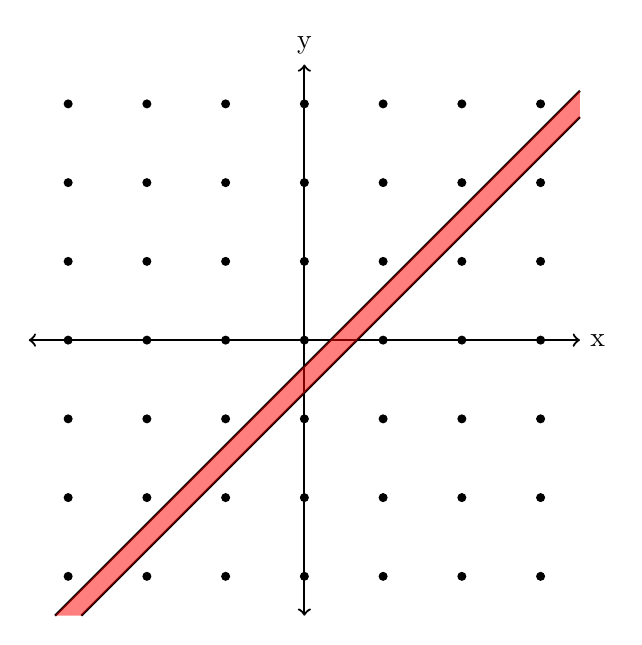
\begin{tikzpicture}
    %\draw[style=help lines,very thin] (-4, -4) grid (4, 4);
    \foreach \x in {-3, -2, ..., 3} {
      \foreach \y in {-3, -2, ..., 3} {
        \node[draw, circle, fill=black, inner sep=1pt] at (\x, \y) {};
      }
    }

    \draw[thick, ->] (0, 0) -- (3.5, 0) node[anchor=west] {x};
    \draw[thick, ->] (0, 0) -- (0, 3.5) node[anchor=south] {y};
    \draw[thick, ->] (0, 0) -- (-3.5, 0);
    \draw[thick, ->] (0, 0) -- (0, -3.5);


    \coordinate (C1LEFT) at (-3.167, -3.5);
    \coordinate (C1RIGHT) at (3.5, 3.167);
    \coordinate (C2LEFT) at (-2.833, -3.5);
    \coordinate (C2RIGHT) at (3.5, 2.833);
    \draw[thick] (C1LEFT) -- (C1RIGHT);
    \draw[thick] (C2LEFT) -- (C2RIGHT);
    \fill[fill=red, opacity=0.5]
      (C1LEFT) -- (C1RIGHT) -- (C2RIGHT) -- (C2LEFT) -- cycle;
  \end{tikzpicture}

  \label{bbloop}
  \caption{Solutions of the problem
           \ref{pbloop}. The solutions of the relaxation lie in the red area.}
\end{figure}

In this case, the problem is unbounded and makes the branch-and-bound algorithm
loop. This is why we will try to add to the original problem $S$ constraints of
the form $$-B \leqslant x_i \leqslant B$$

for all variables $x_i$ to obtain a bounded problem $S'$.
Moreover, we want to choose the bound $B$ such that
the bounded problem $S'$ is satisfiable if and only if the problem $S$
is satisfiable \footnote{We will call solutions of such a bounded
problem \textit{solutions of small size.}}. 
This is what we are going to see in the next section.

\subsection{Obtaining Bounds for ILPs and MILPs}
\label{schrijverbnd}
First of all, let us remark that if a linear problem contains only 
large inequalities, it could be put in the form:

\begin{displaymath}
  \left\{
  \begin{array}{ccccccl}
    a_{11} x_1 & + & ...    & + & a_{1n} x_n & \leqslant & b_1 \\
               &   & \ddots &   &            &           &     \\
    a_{p1} x_1 & + & ...    & + & a_{pn} x_n & \leqslant & b_p \\
  \end{array}
  \right.
\end{displaymath}

or in the matrix form $Ax \leqslant b$ with
$$A = (a_{ij})_{\substack{1 \leqslant i \leqslant n \\
                          1 \leqslant j \leqslant p}}$$
                          
and
$b = (b_j)_{1 \leqslant j \leqslant p}$. We identify a valuation of $n$
variables to a vector of dimension $n$.

Now, we are going to give the outline of a proof that MILPs admit a solution
if and only if they admit a solution of small size. In what follows, we will
focus on ILPs, but the result can be easily extended to MILPs. Most of the
definitions and results can be found in Schrijver's book
\cite[Sections 7 and 16]{Schrijver1998}.

\begin{definition}[Finitely Generated Cone]
  A set of points $C$ is a \textup{finitely generated cone}
  \ifff{} $C = \cone~\{x_0, ..., x_{n-1}\}$ where
  $$\cone~\{x_0, ..., x_{n-1}\} =
      \left\{\sum_{i=0}^{n-1} \lambda_i x_i~|~
               \lambda_0, ..., \lambda_{n-1} \geqslant 0\right\}
  $$

  for some $x_0, ..., x_{n-1}$.
\end{definition}

\begin{definition}[Polyhedral Cone]
  A set of points $C$ is a \textup{polyhedral cone}
  \ifff{} $C = \{x~|~Ax \leqslant 0\}$ for some matrix $A$.
\end{definition}

\begin{theorem}[Farkas-Minkowsky-Weyl Theorem]
  A set $C$ is a finitely generated cone \ifff{} it is a polyhedral cone.
\end{theorem}

\begin{definition}[Polyhedron]
  A set of points $P$ is a \textup{convex polyhedron} \ifff{}
  $$P = \{x~|~Ax \leqslant b\}$$

  for some matrix A and vector b.
\end{definition}

Note that a polyhedron could be interpreted as the set of solutions of a linear
problem with only non-strict inequalities.

\begin{definition}[Polytope]
  A set of points $P$ is a \textup{polytope} \ifff{} it is the convex hull of a
  finite set $C = \{x_0, ..., x_{m-1}\}$, \textit{i.e}
  $$P = \left\{
    \sum_{i=0}^{m-1} \lambda_i x_i~|~\lambda_0, ..., \lambda_{m-1} \geqslant 0
                                  \wedge \sum_{i=0}^{m-1} \lambda_i = 1
        \right\}$$

  We will also use the following notation: $P = \hull~C$.
\end{definition}

\begin{corollary}[Decomposition Theorem for Polyhedra]
  A set of points $P$ is a polyhedron \ifff{} there exists a polytope $Q$ and a
  finitely generated cone $C$ such that $P = Q + C$.
\end{corollary}

To illustrate this theorem, let us take the following problem:
\begin{equation} \label{eqdecomp}
  \left\{
  \begin{array}{rcccc}
    -6x & + & 2y & \leqslant & 1  \\
    3x  & + & 2y & \geqslant & 11 \\
        &   & 2y & \geqslant & 1  \\
    2x  & - & 4y & \leqslant & 5
  \end{array}
  \right.
\end{equation}

According to the theorems, the set of the solutions of this problem is a
polyhedron. The decomposition of this polyhedron is represented in figure
\ref{figdecomp}.

\begin{figure}[h]
  \label{figdecomp}
  \centering

  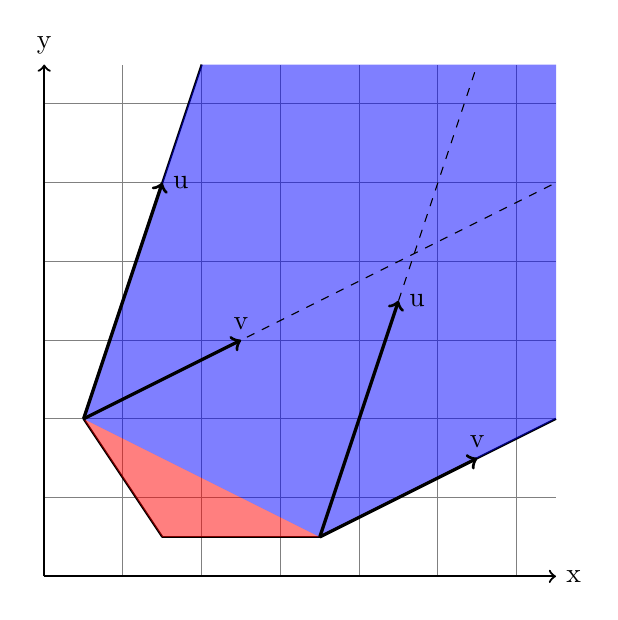
\begin{tikzpicture}
    \coordinate (extr) at (6.5, 6.5);
    \draw[style=help lines, thin] (0, 0) grid (extr);
    \draw[thick, ->] (0, 0) -- (6.5, 0) node[anchor=west] {x};
    \draw[thick, ->] (0, 0) -- (0, 6.5) node[anchor=south] {y};

    \coordinate (A) at (2, 6.5);
    \coordinate (B) at (0.5, 2);
    \coordinate (C) at (1.5, 0.5);
    \coordinate (D) at (3.5, 0.5);
    \coordinate (E) at (6.5, 2);
    \coordinate (B') at (6.5, 5);
    \coordinate (D') at (5.5, 6.5);
    \draw[thick] (A) -- (B);
    \draw[thick] (B) -- (C);
    \draw[thick] (C) -- (D);
    \draw[thick] (D) -- (E);
    \fill[fill=red, opacity=0.5] (B) -- (C) -- (D) -- cycle;
    \fill[fill=blue, opacity=0.5] (A) -- (B) -- (D) -- (E) -- (extr) --
                                  cycle;

    \draw[very thick, ->] (B) -- (1.5, 5) node[anchor=west] {u};
    \draw[very thick, ->] (B) -- (2.5, 3) node[anchor=south] {v};
    \draw[very thick, ->] (D) -- (4.5, 3.5) node[anchor=west] {u};
    \draw[very thick, ->] (D) -- (5.5, 1.5) node[anchor=south] {v};
    \draw[dashed] (B) -- (B');
    \draw[dashed] (D) -- (D');
  \end{tikzpicture}

  \caption{Decomposition of the polyhedron defined by the problem
           \ref{eqdecomp}. The polyhedron is represented by the
           red and blue areas. As we can see, it is the sum of a polytope
           (the red triangle) and a cone ($\cone~\{u, v\}$).
          }
\end{figure}

\begin{corollary}
  $P$ is a polytope \ifff{} $P$ is a bounded polyhedron.
\end{corollary}

\begin{definition}[Integer Hull]
  Given a polyhedron $P$, the \textup{integer hull} $P_I$ is the convex hull of
  the integral vectors of $P$, i.e $P_I = \hull (P \cap \ints^n\}$.
\end{definition}

\begin{theorem}[Meyer, 1974]
\label{meyer theorem}
  For any rational polyhedron $P$, $P_I$ is a polyhedron. Moreover, if
  $P = Q + C$ with $Q$ a polytope and $C$ a cone, then there exists a polytope
  $Q'$ such that $P_I = Q' + C$.
\end{theorem}
\begin{proof}
  Let us decompose $P$ into $P = Q + C$ where
  $C = \cone~\{y_0, ..., y_{s-1}\}$. All the $y_i$'s are rational vectors.
  Without loss of generality we can assume that the $y_i$'s are integral.

  Let us define
  $$D = \left\{\sum_{i=0}^{s-1} \mu_i y_i~|~
               0 \leqslant \mu_i \leqslant 1\right\}$$

  and show that $$P = (Q + D)_I + C$$

  The easy inclusion is the following:
  $$(Q + D)_I + C \subseteq P_I + C = P_I + C_I \subseteq (P + C)_I = P_I$$

  To prove the other inclusion, let us introduce $x \in P$.
  There exists $q \in Q$ and $\lambda_0, ..., \lambda_{s-1}
  \leqslant 0$ such that: $$x = q + \sum_{i < s} \lambda_i y_i$$
  
  But for every
  $i$, $\lfloor \lambda_i \rfloor y_i$ is an integral vector, so
  $$x - \sum_{i<s} \lfloor \lambda_i \rfloor y_i=
      q + \sum_{i<s} (\lambda_i - \lfloor \lambda_i \rfloor) y_i$$

  is integral, and as $\sum_{i<s} (\lambda_i - \lfloor \lambda_i \rfloor) y_i$
  is contained in $D$:
  $$x - \sum_{i<s} \lfloor \lambda_i \rfloor y_i \in (Q + D)_I$$

  Finally: $$x \in (Q + D)_I + C$$

  $(Q + D)$ is bounded, so $(Q + D)_I$ is the convex hull of a finite set, it is
  a polytope. If we take $Q' = (Q + D)_I$, we have the result.
\end{proof}

A graphical representation of this proof is given in figure
\ref{integer_hull_decomp}, with again the polytope defined by the problem
\ref{eqdecomp}. As we can see, $(Q + D)_I + C$ (the
green and yellow areas) is exactly the integer hull of the polyhedron.

\begin{figure}[h]
  \label{integer_hull_decomp}
  \centering

  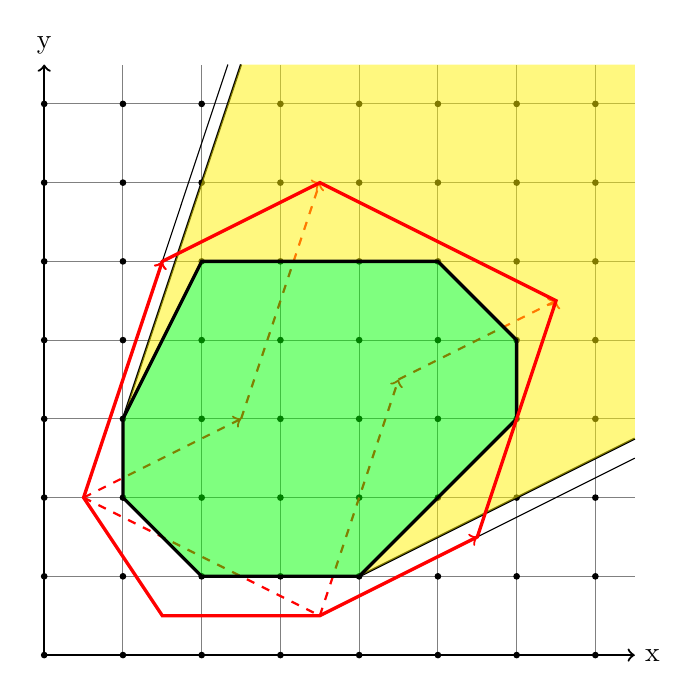
\begin{tikzpicture}
    \coordinate (extr) at (7.5, 7.5);
    \draw[style=help lines, thin] (0, 0) grid (extr);
    \draw[thick, ->] (0, 0) -- (7.5, 0) node[anchor=west] {x};
    \draw[thick, ->] (0, 0) -- (0, 7.5) node[anchor=south] {y};
    \foreach \x in {0, 1, ..., 7} {
      \foreach \y in {0, 1, ..., 7} {
        \node[draw, circle, fill=black, inner sep=0.7pt] at (\x, \y) {};
      }
    }

    \coordinate (A) at (2.333, 7.5);
    \coordinate (A') at (2.5, 7.5);
    \coordinate (B) at (0.5, 2);
    \coordinate (C) at (1.5, 0.5);
    \coordinate (D) at (3.5, 0.5);
    \coordinate (E) at (7.5, 2.5);
    \coordinate (E') at (7.5, 2.75);

    % Extremal points of (Q + D)
    \coordinate (B') at (1.5, 5);
    \coordinate (B'') at (3.5, 6);
    \coordinate (D') at (5.5, 1.5);
    \coordinate (D'') at (6.5, 4.5);

    % Extremal points of (Q + D)_I
    \coordinate (I) at (2, 5);
    \coordinate (J) at (1, 3);
    \coordinate (K) at (1, 2);
    \coordinate (L) at (2, 1);
    \coordinate (M) at (4, 1);
    \coordinate (N) at (6, 3);
    \coordinate (O) at (6, 4);
    \coordinate (P) at (5, 5);

    % Drawing the polytope Q + C
    \draw[thin] (A) -- (B);
    \draw[thin] (B) -- (C);
    \draw[thin] (C) -- (D);
    \draw[thin] (D) -- (E);

    % Drawing lines of the polytope (Q + D)_I + C
    \draw[thick] (A') -- (J);
    \draw[thick] (M) -- (E');

    \draw[red, thick, dashed, ->] (B) -- (B');
    \draw[red, thick, dashed, ->] (B) -- (B');
    \draw[red, thick, dashed, ->] (B) -- (2.5, 3);
    \draw[red, thick, dashed, ->] (B') -- (B'');
    \draw[red, thick, dashed, ->] (2.5, 3) -- (B'');
    \draw[red, thick, dashed, ->] (D) -- (D');
    \draw[red, thick, dashed, ->] (D) -- (4.5, 3.5);
    \draw[red, thick, dashed, ->] (D') -- (D'');
    \draw[red, thick, dashed, ->] (4.5, 3.5) -- (D'');
    \draw[red, thick, dashed] (B) -- (D);
    \fill[fill=yellow, opacity=0.5]
      (A') -- (J) -- (I) -- (P) -- (O) -- (N) -- (M) -- (E') -- (extr)
           -- cycle;
    \draw[very thick, fill=green, fill opacity=0.5]
      (I) -- (J) -- (K) -- (L) -- (M) -- (N) -- (O) -- (P) -- cycle;
    \draw[red, very thick]
      (B'') -- (B') -- (B) -- (C) -- (D) -- (D') -- (D'') -- cycle;
  \end{tikzpicture}

  \caption{Decomposition of the integer hull of the polytope defined by the
           problem \ref{eqdecomp}.
           The boundary of the set $(Q + D)$ is represented
           in red and $(Q + D)_I$ is represented in green.}
\end{figure}

\pagebreak

\textbf{Remark:}
Using the notations of the previous proof:
\begin{displaymath}
  P \cap \ints^n \neq \emptyset \Longleftrightarrow
  P_I \neq \emptyset            \Longleftrightarrow
  (Q + D)_I \neq \emptyset      \Longleftrightarrow
  (Q + D) \cap \ints^n \neq \emptyset
\end{displaymath}

Hence, there is an integral point in the polyhedron $P$ \ifff{} there is an
integral point in the (bounded) polytope $(Q + D)$.
What remains to do is to find a bound $B$ that depends on the
parameters of the problem. To do so, a solution is to generalize the previous
theorems to incorporate bounds. We will use the notation
$\llbracket a, b \rrbracket$ for the set of integers in the interval $[a, b]$.

\begin{theorem}[Generalized Farkas-Minkowsky-Weyl Theorem]
  A set $C$ is a finitely generated cone \ifff{} it is a polyhedral cone.

  Moreover, if $C = \{x~|~Ax \leqslant 0\}$ and
  $A \in \llbracket -m, m \rrbracket^{p \times n}$ with $m \geqslant 1$,
  there exists a finite set $Y$ such that
  $Y \subseteq \llbracket -B, B \rrbracket^n$
  and $$C = \cone~Y$$
  
  where
  $$B = (n - 1)! \cdot m^{n-1}$$
\end{theorem}

\begin{corollary}[Generalized Decomposition Theorem]
  A set of points $P$ is a polyhedron \ifff{} there exists a polytope $Q$ and a
  finitely generated cone $C$ such that $P = Q + C$.

  Moreover, if $P = \{x~|~Ax \leqslant b\}$ with
  $A \in \llbracket -m, m \rrbracket^{p \times n}$,
  $b \in \llbracket -m, m \rrbracket^p$, and $m \geqslant 1$,
  then there exist finite sets
  $Q \subseteq [-B, B]$ and $X \subseteq \llbracket -B, B \rrbracket$ such that
  $$P = \hull~Q + \cone~X$$
  
  with $$B = n! \cdot m^n$$
\end{corollary}

We finally have the desired result:

\begin{corollary}[Existence of small solutions for ILPs]
  \label{small-ilp}
  If $P = \{x~|~Ax \leqslant b\}$ with
  $A \in \llbracket -m, m \rrbracket^{p \times n}$,
  $b \in \llbracket -m, m \rrbracket^p$ and $m \geqslant 1$, then
  $$P \cap \ints^n \neq \emptyset \Longleftrightarrow
  P \cap \llbracket -B, B \rrbracket^n \neq \emptyset$$
  
  where
  $$B = (n + 1)! \cdot m^n$$
\end{corollary}

With the same outline of proof, we can obtain a more general result that
encompasses MILPs and strict inequalities. 

\begin{theorem}[Existence of small solutions for MILPs]
  \label{small-milp}
  If $I$ is a subset of $\llbracket 1, n \rrbracket$ and
  $$P = \{x~|~Ax \leqslant b \wedge A'x < b'\}$$
  
  with
  $A \in \llbracket -m, m \rrbracket^{p \times n}$,
  $b \in \llbracket -m, m \rrbracket^p$,
  $A' \in \llbracket -m, m \rrbracket^{p' \times n}$,
  $b' \in \llbracket -m, m \rrbracket^{p'}$ and $m \geqslant 1$, then

  $$\{x \in P~|~\forall x_i \in I.~x_i \in \ints\} \neq \emptyset
      \Longleftrightarrow
    \{x \in P~|~\forall x_i \in I.~x_i \in \llbracket -B, B \rrbracket\}
      \neq \emptyset$$

  where
  $$B = (n + 1)! \cdot m^n$$
\end{theorem}

\textbf{Remark:} If we take the previously defined bound $B$:
$$\log B \approx n \log n + n \log m$$

Hence, the number of bits
necessary to represent numbers in the interval $\llbracket -B, B \rrbracket$
is polynomial in the size of the input. Therefore, a small solution $v$ to
an ILP can be used as a certificate of polynomial size, so ILPs are NP.

\pagebreak

\section{Formalization in Isabelle}
\label{secformalization}

As we have presented a method to solve MILPs, we can focus on its
formalization, which has been the main part of the work during this internship.
It consisted in the formalization of Schrijver results concerning linear
inequalities as described in section \ref{forlineq}), then in the
implementation and the proof of correction of the branch-and-bound algorithm
as described in section \ref{forbb}.

\subsection{Formalization of Schrijver's Results concerning Linear
            Inequalities}
\label{forlineq}
This part is about the formalization of the results from Schijver's book
described in section \ref{schrijverbnd} in Isabelle.
Also, other results including Farkas' lemma and the Carathéodory's theorem
have been formalized.
In total, 5551 lines of proofs were written. The work was published in the
\textit{Archive for Formal Proofs} (AFP), a collection of proof libraries in
Isabelle \cite{Linear_Inequalities-AFP}.
This was done in collaboration with René Thiemann and Ralph Bottesch:
\begin{itemize}
  \item René included bounds for the various operations that are performed 
  when executing the decomposition theorem.  He also verified
    Theorem~\ref{meyer theorem} of Meyer. 
  \item Ralph and René formalized the fundamental theorem of linear
    inequalities.
  \item I mainly focused on the demonstration of the Farkas-Minkowsky-Weyl and
    the decomposition theorem.
\end{itemize}


The formalization follows the outline given in section \ref{schrijverbnd}.
Several theorems, for example the Farkas-Minkowsky-Weyl theorem, have a general
formulation:
\Snippet{farkas-minkowsky}
and particular formulations including bounds:
\Snippet{farkas-minkowsky-2}
where the following Isabelle notations are used:
\begin{itemize}
  \item $\mathtt{carrier\_vec}~n$ is the set of vectors $\mathbb{K}^n$
    where $\mathbb{K}$ is a field.
  \item $\mathtt{carrier\_mat}~n_r~n_c$ is the set of matrices
    $\mathbb{K}^{n_r \times n_c}$.
  \item $\mathbb{Z}_v$ is the set of integral vectors.
  \item $\mathbb{Z}_m$ is the set of integral matrices.
  \item $\mathtt{Bounded\_vec}~B$ is the set of vectors with coefficients in
    the interval $[-B, B]$.
  \item $\mathtt{Bounded\_mat}~B$ is the set of matrices with coefficients in
    the interval $[-B, B]$.
  \item $\mathtt{det\_bound}~n~m$ is $n! \cdot m^n$.
\end{itemize}

A difficulty I was confronted with is the variety of definitions for linear
combinations in Isabelle. The standard definition is
$$\mathtt{lincomb}~c~V = \sum_{v \in V} c(v) \cdot v$$

where $V$ is a set of vectors and $c$ is a map from vectors to scalars.

A problem that can occur is the distributivity when we multiply this sum by
a matrix. Indeed, it is clear that
$$A \sum_i \lambda_i x_i = \sum_i \lambda_i \cdot A x_i.$$

But this equality
cannot be simply stated with the operator $\mathtt{lincomb}$ Indeed, it is
possible that there exist two vectors $x_0$ and $x_1$ such that
$A x_0 = A x_1$. If we want to express $\sum_i \lambda_i \cdot A x_i$ using
$\mathtt{lincomb}$, then the scalar coefficient associated to $A x_0$ is
neither $c(x_0)$ nor $c(x_1)$ but $\sum_{x . A x = A x_0} c(x)$,
which is more complicated to work with. More generally, this problem occurs
every time we want to prove the equality
$$f(\sum_i \lambda_i x_i) = \sum_i \lambda_i f(x_i)$$

where $f$ is a linear map.

A solution to tackle this problem is to use linear combinations over lists,
defined this way:
$$\mathtt{lincomb\_list}~c~\mathtt{Vs} = \sum_{i = 0}^{l-1} c(i) \cdot v_i$$

where $\mathtt{Vs} = [v_0, ..., v_{l-1}]$ is a list of vectors and $c$ is a
function mapping integers to scalars. 

This way, the distributivity of a linear map to a linear combination can be
expressed in a direct manner. To use the advantages of both definitions, we
usually define our concepts in two manners: one using sets and the other using
lists. For example, here is how non-negative linear combinations are defined,
for sets and for lists:
\Snippet{nonneg-lincomb}
\Snippet{nonneg-lincomb-list}
where $\mathtt{c}~`~\mathtt{Vs} = \{\mathtt{c}(x)~|~x \in \mathtt{Vs}\}$
is the image of the set $\mathtt{Vs}$ under $\mathtt{c}$.

We can then use this definition to define convex combinations:
\Snippet{convex-lincomb}
\Snippet{convex-lincomb-list}
and then define convex hulls:
\Snippet{convex-hull}
\Snippet{convex-hull-list}
Finally, we can show that these two definitions are equivalent:
\Snippet{convex-hull-equivalence}

\subsection{Formalization of a Branch-and-Bound Algorithm}
\label{forbb}

The next part is the formalization of a branch-and-bound algorithm, as
described in the section \ref{bbdescr}. The idea was to state and prove the
correctness of a simple algorithm, without any optimization.

I first developped a function $\mathtt{branch\_and\_bound\_core}$ that takes
four arguments:
\begin{itemize}
  \item A list of linear constraints \texttt{cs}.
  \item A list of variables \texttt{Is} required to be integral.
  \item A function \texttt{lb} mapping variables of \texttt{Is} to integral
    lower bounds.
  \item A function \texttt{ub} mapping variables of \texttt{Is} to integral
    upper bounds.
\end{itemize}
It returns either $\mathtt{Some}~v$ is a solution $v$ within the bounds is
found, or $\mathtt{None}$.
The code of this function can be found in appendix \ref{bbcode}

The goal of the arguments \texttt{lb} and \texttt{ub} is to bound the problem.
This way, I ensure that this function always terminates. To do so, a
convenient way in Isabelle is to use a \textit{measure}. It is function mapping
the arguments of the function \texttt{f} to natural numbers. If we prove that
at each recursive call the measure strictly decreases, then
an infinite sequence of recursive calls cannot happen and the function always
terminates. The measure I used is the following:
$$
\max\left(
     0,
     \sum_{x_i \in \mathtt{Is}} (\mathtt{ub}(x_i) - \mathtt{lb}(x_i))
     \right)
$$

Indeed, if there is a rational solution $v$ that is not a mixed-integer
solution, then $\sum (\mathtt{ub}(x_i) - \mathtt{lb}(x_i)) > 0$.
Furthermore, if $v(x_i) \notin \ints$, if we do a recursive call with
$\mathtt{ub}(x_i)$ substituted by $\lfloor v(x_i) \rfloor$, as
$v(x_i) \leqslant \mathtt{ub}(x_i)$,
$\lfloor v(x_i) \rfloor < \mathtt{ub}(x_i)$ so the measure strictly decreases
at the recursive calls. The same happens if $\mathtt{lb}(x_i)$ is substituted
by $\lceil v(x_i) \rceil$.

Once the termination proved, I proved correctness properties, the first is that
if a valuation is found, it satisfies the MILP:
\Snippet{bbcore-sat}
and the other is that if no valuation is found, then there is no valuation
\texttt{v} that satisfies the MILP and such that the valuations of the integral
variables are bounded by \texttt{lb} and \texttt{ub}:
\Snippet{bbcore-unsat}
where the Isabelle notation $v \vDash_{mcs} (S, I)$ is equivalent to notation
$v \vDash_I S$.

The goal now is to use the theorem \ref{small-milp} to have a formalized
complete solver for MILPs. The problem is that linear constraints are coded
with a datastructure called \textit{linear polynomials} that should be
converted to the form of vectors and matrices to use the theorem.

To do so, linear constraints are converted to the type \texttt{Le\_Constraint}
that is more practical to use, as the description of different inequalities uses
a sum-type with only two constructors instead of ten for the type
\texttt{constraint}. Indeed, I first tried to express the conversion using
directly the standard type, and when I switched to \texttt{Le\_Constraint}'s, I
considerably simplified the proofs (around 80 lines of proof were saved).
%The conversion theorem is the following:
%\Snippet{mats-vecs-of-constraints}

Afterwards, some work to convert rational constraints to integral constaints
is needed. 
I use it to define a function \texttt{compute\_bound} that maps a list of
constraints to the desired bound. I prove that:
\Snippet{compute-bound}

Finally, I am able to state a complete MILP-solver based on the
branch-and-bound algorithm:
\Snippet{branch-and-bound}
and to prove its correction:
\Snippet{branch-and-bound-sat}
\Snippet{branch-and-bound-unsat}

In total, the formalization of this algorithm takes 1062 lines of code.
It can be consulted in at:
\url{https://github.com/Cemoixerestre/MILP-Isabelle}.

\section{Future Work}
\label{secfuture}

Even if I have written and proved the correctness of a branch-and-bound
algorithm, the work is not yet finished. Indeed, some tasks are needed before
having a more effective formalized MILP-solver with an incremental interface.
Here is the prospective work to complete the project.

\subsection{Using the Incremental Interface}
We can remark that for the branch-and-bound algorithm, at the branching step,
we only try to solve problems with a single constraint added to the original
problem. This is why it should be interesting to use the incremental interface
described in \cite{Thiemann2018, BHT2019}. In the current implementation,
the computation (including the preprocessing steps) is always made from
scratch. The difficulty is that in the current interface, the internal state is
initialized with a (finite) list of constraints, and only constraints of this
list can be asserted. To efficiently use the incrementality, this interface
should be upgraded so that arbitrary constraints can be asserted.

\subsection{Gomory Cuts}

Suppose that a valuation $v$ such that $v \vDash S$ has been found but that
$v \not{\vDash_I} S$. A \textit{cut} is a
linear constraint $c$ such that $v$ does not satisfy $c$ but for every
mixed-integer solution $v'$, $v'$ satisfies $c$. The goal of a cut is
to prune non-integral solutions of the problems while keeping the same integral
solutions.

For example, let us take the following problem:
\begin{equation}
  \label{cuteq}
  \left\{
  \begin{array}{rcccc}
     2x & + & 10y & \geqslant & 5 \\
    -2x & + & 10y & \leqslant & 5
  \end{array}
  \right.
  %\right|
  %x, y \in \ints
\end{equation}

$(0, \frac{1}{2})$ is a non-integral solution. But we can remark that the
following constraint $$x \geqslant \frac{5}{2}$$

is satisfied by all of the
solutions of the problem, but not by $(0, \frac{1}{2})$. We will call this
constraint the \textit{cut}. A graphical representation can be found in figure
\ref{cutfig}.

\begin{figure}[h]
  \label{cutfig}
  \centering

  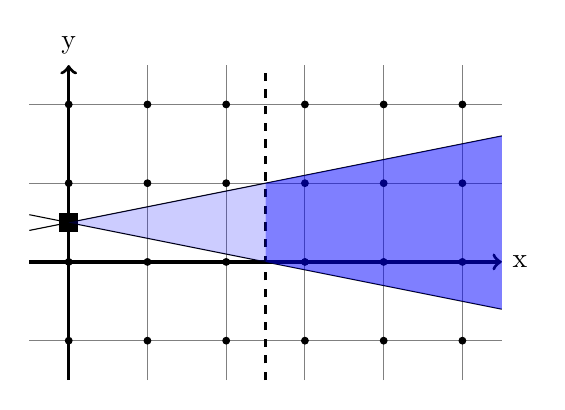
\begin{tikzpicture}
    \coordinate (lextr) at (-0.5, -1.5);
    \coordinate (rextr) at (5.5, 2.5);
    \draw[style=help lines, thin] (lextr) grid (rextr);
    \draw[very thick, ->] (0, -1.5) -- (0, 2.5) node[anchor=south] {y};
    \draw[very thick, ->] (-0.5, 0) -- (5.5, 0) node[anchor=west] {x};
    \foreach \x in {0, 1, ..., 5} {
      \foreach \y in {-1, 0, ..., 2} {
        \node[draw, circle, fill=black, inner sep=0.85pt] at (\x, \y) {};
      }
    }

    \coordinate (A) at (5.5, -0.6);
    \coordinate (B) at (0, 0.5);
    \coordinate (C) at (5.5, 1.6);
    \coordinate (A') at (-0.5, 0.6);
    \coordinate (C') at (-0.5, 0.4);
    \coordinate (A'') at (2.5, 0);
    \coordinate (C'') at (2.5, 1);
    \coordinate (D) at (2.5, -1.5);
    \coordinate (E) at (2.5, 2.5);

    \draw (A) -- (A');
    \draw (C) -- (C');
    \draw[very thick, dashed] (D) -- (E);
    \node[draw, fill=black] at (B) {};

    \fill[fill=blue, opacity=0.5]
      (A) -- (A'') -- (C'') -- (C) -- cycle;
    \fill[fill=blue, opacity=0.2]
      (A'') -- (B) -- (C'') -- cycle;
  \end{tikzpicture}

  \caption{Solutions of the problem \ref{cuteq}.
          The solutions to the problem satisfying the cut lie in the dark blue
          area. The other solutions lie in the light blue area.
          }
\end{figure}

A general method to obtain cuts is described in \cite[Section 4]{Dutertre2006}.
These cuts are called \textit{Gomory cuts}. The combination of the
branch-and-bound algorithm with cut generation is called
\textit{branch-and-cut} and it experimentally outerforms the branch-and-bound
algorithm \cite{Ongoing2012}.

We plan to incorporate Gomory cuts in this branch-and-bound algorithm,
and to prove its correction. As in the previous section, it would
be useful to extend the following interface so that arbitrary constraints (such
as Gomory cuts) could be asserted.

\subsection{Finalization}
As a least contribution, the branch-and-cut function should be extended to an
incremental interface similar to the existing interface for linear problems so
that it could be used efficiently by a SMT-solver.

Also, René has already started to export the code to measure its execution
time. It could be interesting to measure the difference obtained by each of the
previously described optimizations. Finally, it is planned to publish this
work in AFP.

\pagebreak

\section*{Conclusion}
During this internship, I contributed to formalize in Isabelle results about
linear inequalities with René Thiemann and Ralph Bottesch. I used these results
to prove the termination of a branch-and-bound algorithm to solve MILPs. I also
proved the correctness of this algorithm.

This is the first step to extending a verified linear arithmetic solver to
mixed-integer linear arithmetic, with an incremental interface so that it could
be plugged in a SMT-solver.

\bibliographystyle{plain}
\bibliography{sources}

\appendix

\section{Example: an Execution of DPLL($T$)}
\label{dpll}
Let us solve the following SMT-instance (based on linear arithmetic):
$$\Phi \equiv (A \vee B \vee C) \wedge (\neg A \vee B) \wedge
              (\neg A \vee C \vee D) \wedge (\neg C \vee D)$$

with
\begin{displaymath}
\begin{array}{cclcccc}
  A & \equiv & (x & + & y & \geqslant & 3) \\
  B & \equiv & (x &   &   & \leqslant & 1) \\
  C & \equiv & (  &   & y & \leqslant & 1) \\
  D & \equiv & (y & - & x & <         & 2) \\
\end{array}
\end{displaymath}

using DPLL($T$). First, let us interpret $\Phi$ as a SAT-formula and find an
valuation that satisfies it. For example:
\begin{itemize}
  \item Arbitrarily affect the variable $A$ to 1. Assert the atom $A$. Get a
    checkpoint $c_1$.
  \item To solve the clause $(\neg A \vee B)$, we must affect the variable $B$
    to 1. Assert the atom $B$. Get a checkpoint $c_2$.
  \item Affect the variable $C$ to 1. Assert the atom $C$. Get a checkpoint
    $c_3$.
  \item To solve the clause $(\neg C \vee D)$, we must affect the variable $D$
    to 1. Assert the atom $D$. Get a checkpoint $c_4$.
\end{itemize}

Now, we have found an valuation that satisfies $\Phi$ interpreted as a
SAT-formula. But we need to check if this valuation is compatible with an
assignment in the theory of linear arithmetic. It means that we need to find an
assignment to the conjunction $A \wedge B \wedge C \wedge D$, which is equivalent
to the system:
\begin{displaymath}
  \left\{
  \begin{array}{cccccc}
    x  & + & y & \geqslant & 3 & (A) \\
    x  &   &   & \leqslant & 1 & (B) \\
       &   & y & \leqslant & 1 & (C) \\
    y  & - & x & <         & 2 & (D) \\
  \end{array}
  \right.
\end{displaymath}

But this system has no solution. The procedure $\icheck$ may retun that the
constraints $A$, $B$ and $C$ are mutually incompatible. As these three
constraints cannot be satisfied simultaneously, any assignment that satisfies
$\Phi$ must violate at least one of these constraints, so we can deduce that
the clause $(\neg A \vee \neg B \vee \neg C)$ is true. Instead of solving
$\Phi$, we will try to solve the formula
$$\Phi' = \Phi \wedge (\neg A \vee \neg B \vee \neg C)$$

We need to backtrack, but we can notice that we could bactrack just before
the choice to affect $C$ to 1 was made. So let us backtrack to $c_2$, where
only the variables $A$ and $B$ are affected.

\begin{itemize}
  \item To solve the clause $(\neg A \vee \neg B \vee \neg C)$, we must affect
    the variable $C$ to 0. Assert the atom $\neg C$. Get a checkpoint $c'_3$.
  \item To solve the clause $(\neg A \vee C \vee D)$, we must affect the
    variable $D$ to 1. Assert the atom $D$. Get a checkpoint $c'_4$.
\end{itemize}

Again, we have a valuation that satisfies $\Phi'$ interpreted as a
SAT-formula. We have to find an assignment that satisfies the conjunction
$A \wedge B \wedge \neg C \wedge D$, which is equivalent to the system:
\begin{displaymath}
  \left\{
  \begin{array}{cccccc}
    x  & + & y & \geqslant & 3 & (A) \\
    x  &   &   & \leqslant & 1 & (B) \\
       &   & y & >         & 1 & (\neg C) \\
    y  & - & x & <         & 2 & (D) \\
  \end{array}
  \right.
\end{displaymath}

$\icheck$ may return the assignment $(x=1, y=2)$. Finally, the formula $\Phi$
is satisfiable, and $(x=1, y=2) \vDash \Phi$.

\section{Code of the Core of the Branch-and-Bound Procedure}
\label{bbcode}

\Snippet{bbcore}
To understand the code:
\begin{itemize}
  \item \texttt{bounds\_to\_constraints Is lb ub} returns a list containing the
    constraints $x_i \geqslant \mathtt{lb}~x_i$ and
    $x_i \leqslant \mathtt{ub}~x_i$ for all elements $x_i$ of the list
    \texttt{Is}.
  \item `` \texttt{@} '' is the symbol used for list concatenation. In this case,
    \linebreak \texttt{cs @ bounds\_to\_constraints Is lb ub} is the list
    composed by the constraints of \texttt{cs} and of
    \texttt{bounds\_to\_constraints~Is~lb~ub}.
  \item The function \texttt{simplex} takes as arguments a list of
    constraints and returns \texttt{Unsat} if there is no rational solution to
    this combination of constraints, or \texttt{Sat v} such that
    $\langle \mathtt{v} \rangle$ is a rational valuation satisfying these
    constraints.
  \item The function \texttt{find} takes as arguments a predicate \texttt{f}
    and a list \texttt{Is} and returns $\mathtt{Some}~x_i$ where $x_i$ is
    an element of \texttt{Is} such that $\mathtt{f}~x_i$ is true, or
    \texttt{None} if no such element exists.
\end{itemize}

\end{document}
